%\setchapterpreamble[u]{%
%\dictum[Albert Einstein]{Probleme kann man niemals mit derselben Denkweise lösen, durch die sie entstanden sind.}
%}

\chapter{Grundlagen der HDR-Bilder}
\label{chap:hdr}


In den vergangenen Jahren hat die digitale Fotografie zu einem Umdenken und einer Neuschaffung von Kommunikationskanälen geführt. Im analogen Zeitalter war Fotografie in erster Linie ein autobiographisches Medium. Fotografien hatten unter anderem eine Daseinsberechtigung im Familien-Fotoalbum als Gedächtnisstütze zu früheren Zeiten.

Durch die Verbreitung von digital Kameras (insbesondere auch solchen die in Smartphones und Handys eingebaut sind) haben Fotografien aber auch eine immer größere Rolle als Kommunikationsmedium eingenommen. 
In diesem Zuge spielt auch die digitale Bildbearbeitung eine immer größer werdende Rolle. 

Bevor auf die Grundlagen von \gls{HDR}-Bildern näher eingegangen wird bedarf es noch zunächst der Schaffung von einigen Grundlagen.

Digital Bilder werden in der heutigen Zeit in der Regel in Form der drei Farbkanäle für Rot, Grün und Blau dargestellt (sog. \gls{RGB-Farbraum}). Häufig kommt noch ein vierter Kanal, der sog. Alpha-Kanal hinzu, der für die Darstellung von Transparenz genutzt wird. 

Diese drei bzw. vier Kanäle werden in der Regel mittels eines Bytes repräsentiert. Damit können 16,7 Millionen verschieden Farben dargestellt werden. Trotz dieser großen Zahl sind nur 256 verschiedene Werte für jeden Farbkanal möglich. Diese Anzahl ist häufig unzureichend Szenen mit hohen Helligkeitsunterschieden zu repräsentieren (vgl. \cite[S.~1f]{Reinhard}).


\begin{figure}[h]
  \begin{center}
    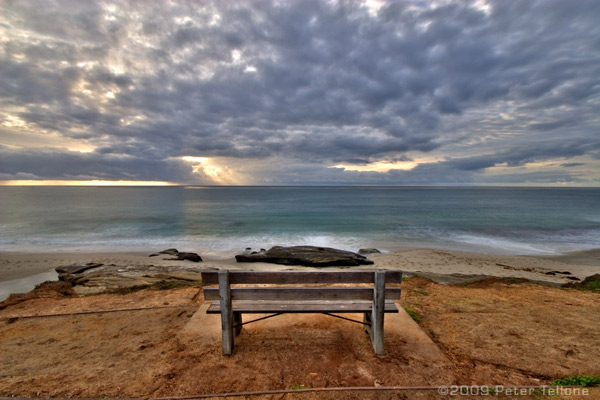
\includegraphics[width=\textwidth]{example}
    \caption{Beispielhaftes \gls{HDR} Bild mit bereits angewandtem Tone-Mapping-Verfahren (siehe \cite{tellone}) }
    \label{fig:teezer}
  \end{center}
\end{figure}

Dieses Problem wird durch die Verwendung von \gls{HDR} Bildern behoben. Ziel ist es mehr Farben und Details in unterschiedlichen Bildbereichen sichtbar zu machen. Um dies zu ermöglichen erhöht man bei \gls{HDR} Bildern den \gls{Dynamikumfang} des Bildbereiches. Dazu bricht man die Beschränkung auf den Byte-Bereich auf und erlaubt Fließkomma-Werte im Bildbereich.

%------------------------------------------------------------------------------------------------------------
\section{Prinzip}

Das menschliche Auge kann in einer täglichen Szene einen \gls{Dynamikumfang} im Bereich von 1:10.000 (vgl. \cite{Fairchild04theicam}) wahrnehmen. Dies liegt weit über den herkömmlichen Werten eines normalen Kamera-Sensors. In der Tabelle \autoref{tab:illumination} können verschiedenen Dynamikumfänge (und die damit zusammenhängende Beleuchtungsstärke) entnommen werden. 
Um wie gewünscht mit \gls{HDR} Bildern einen höheren \gls{Dynamikumfang} darstellen zu können müssen daher mehr Informationen als über den herkömmlichen Weg beschafft werden. Dazu werden entweder mehrere Bilder mit verschiedenen \glspl{Belichtungszeit} zu einer \gls{Radiance Map} kombiniert oder es werden spezielle Kamera-Sensoren eingesetzt, welche in der Lage sind die höhere Dichte der Bildinformationen (z.B. die großen Helligkeitsunterschiede) aufzunehmen (vgl. \cite{Yang99a640}). 


\begin{table}
  \begin{center}
    \begin{tabular}{ccc}
	\toprule
	Umgebung & Beleuchtungsstärke ($cd/m^2$)\\ \midrule
	Sternenhimmel & $10^{-3} $\\	
	Mondschein & $10^{-1} $\\	
	Innenraum Beleuchtung & $10^{2} $\\	
	Sonnenlicht & $10^{5} $\\	
	\midrule
	Herkömmliche Monitore & $10^{2} $\\	
	\bottomrule
    \end{tabular}
    \caption{Beleuchtungsstärken in verschiedenen Umgebungen \cite[S.~6]{Reinhard}}
    \label{tab:illumination}
  \end{center}
\end{table}



Der hier verwendete Begriff des \enquote{\gls{Dynamikumfang}} beschreibt das Verhältnis zwischen hellstem und dunkelstem Pixel im Bild. Um Ausreißer weniger zu berücksichtigen und die Messung robuster zu machen werden hierbei manchmal auch Quantile verwendet die dafür sorgen sollen, dass Rauschen nicht ins Gewicht fällt. Bei Bildschirmen hingegen wird unter dem \gls{Dynamikumfang} das Verhältnis zwischen der maximalen und minimalen Leuchtkraft verstanden (vgl. \cite[S.~4]{Reinhard}.

%------------------------------------------------------------------------------------------------------------

\section{Anwendungsgebiet und Geschichte}

Die Möglichkeiten des Einsatzes von \gls{HDR} Bildern sind vielfältig. Die nachfolgende Liste umfasst einige der Gebiete, in denen diese Technologie eingesetzt wird oder werden kann (vgl. \cite[S.~87f]{Reinhard}).

\begin{description}

\item[Digitale Fotografie:] Die verschiedenen Kamera-Hersteller gehen bereits immer mehr in Richtung der sog. Aufnahme abhängigen Daten. In diesen sind bereits häufig mehr Bildinformationen enthalten. Dabei handelt es sind bei verschiedenen Herstellern in der Regel jedoch auch um verschiedene \gls{RAW} Formate, die meist nicht kompatibel sind. 

\item[Satellitenbilder:] Satellitenbilder beinhalten in aller Regel sehr viel mehr Informationen als nur den sichtbaren Bereich des Lichtspektrums. \gls{HDR} Bilder sind hier von Bedeutung, da sie multispektrale Aufnahmen ermöglichen.

\item[Visualisierungen und Rendering:] Eine der ersten Anwendungen waren vermutlich die ersten Render-Engines von Visualisierungen (Computer-Spiele, Med. Visualisierungen und Simulationen, etc.). Bei manchen Anwendungen ist es insbesondere für Reflektionen wichtig auch nicht sichtbare Frequenzen bei Berechnungen mit einzubeziehen. Da diese durch Interferenzen wieder sichtbar werden können und somit der Detailgrad steigt.

\item[Bildbearbeitungssoftware:] Die großen Bildbearbeitungs-Anwendungen bieten mittlerweile in der Regel auch die Bearbeitung und Generierung von \gls{HDR} Bildern an. Als Beispiele seinen hier Adobe Photoshop\footnote{\url{http://adobe.com/photoshop}}, Photogenics\footnote{\url{http://www.cinepaint.org}} und Photomatix\footnote{\url{http://www.hdrsoft.com/download.html}} genannt.

\item[Medizin:] In der Endoskopie besteht ein hoher Bedarf an immer höher auflösender \gls{CMOS} Bildsensoren. Diese können immer bessere Aufnahmen aus dem Inneren des Körpers liefern und helfen damit in der Medizin große Fortschritte zu machen. Solche Sensoren können bereits in der Größe eines Streichholzkopfes einen Dynamikumfang von 179 dB erreichen (vgl. \cite{Klingler_Richter_Strobel_2006}).

\item[Virtual Reality:] Bei Anwendungen, bei denen sich der Benutzer in einem virtuellen Raum bewegt, wird die Wahrnehmung zunehmend wichtig. Auch hier spielen deshalb hohe Dynamikumfänge eine besondere Rolle. Außerdem ist es besonders in diesem Bereich wichtig gute Kompressions-Algorithmen für \gls{HDR} Bilder zu entwickeln um eine schnelle Übertragung dieser zu gewährleisten. Auch bei dem platzieren von sythetischen Objekten in realen Szenen (vgl. \cite{Debevec:2008:RSO:1401132.1401175}) können \gls{HDR} Bilder eingesetzt werden um dem Betrachter eine noch realere Szene darstellen zu können.
\end{description}

%------------------------------------------------------------------------------------------------------------
\section{Bilderzeugung}
Bei der Erstellung von \gls{HDR} Bildern gibt es unterschiedliche Möglichkeiten. Dabei muss man jedoch zwischen echten \gls{HDR} Bildern und \enquote{Pseudo-\gls{HDR}} Bildern unterscheiden. Im Nachfolgenden werden die verschiedenen Verfahren kurz beschrieben. Der Fokus liegt jedoch auf dem letzten Verfahren, der \nameref{sub:belichtungsreihe}.


\subsection{Pseudo-HDR Bilder}
Bei Pseudo-\gls{HDR} Bildern handelt es sich um eine einfache Fusion von Bildreihen. Deswegen werden diese Verfahren auch Exposure Blending oder Exposure Fusion genannt. Bei dieser Technologie geht es darum mehr Details aus einer Belichtungsreihe von \gls{LDR} Bildern zu generieren, ohne dabei ein \gls{HDR} Bild zu erzeugen (vgl. \cite{Jing_Hong_Zheng_Rahardja_2012}). Die Bilder der Belichtungsreihe werden dazu einfach fusioniert. Diese Technologie wird hier jedoch nicht behandelt.

\subsection{HDR-Kameras} 
Diese speziellen Kameras verfügen über Bildsensoren die von sich aus einen hohen Dynamikumfang aufnehmen können und dadurch bereits die notwendigen Informationen in einer Aufnahme generieren können. Diese Spezial-Kameras sind jedoch noch sehr teuer und wenig verbreitet. (vgl. \cite[S. 95ff]{Bloch2012}). Viele digitale Spiegelreflex-Kameras bieten mittlerweile einen \gls{HDR}-Modus an.

\subsection{HDR-Bildgenerierung aus einer Belichtungsreihe}
\label{sub:belichtungsreihe}
Um ein \gls{HDR} Bild zu aus einer Belichtungsreihe zu erzeugen braucht man zunächst die Grundlage für das Bild. Dazu sind in der Regel mehr Informationen notwendig als eine einzelne Aufnahme liefern kann. Deshalb werden mehrere Bilder der selben Szene mit unterschiedlichen Belichtungszeiten aufgenommen. Ziel der Algorithmen ist es dann anschließend aus diesen Bildern ein \gls{HDR} Bild zu erzeugen.

Um die Bilder später weiter zu verarbeiten müssen diese jedoch zunächst aligniert werden. Dies ist aufgrund der verschiedenen Belichtungswerte der Aufnahmen nicht über Kantendetektionsverfahren möglich, da diese Merkmale unter den unterschiedlichen Belichtungen sehr stark variieren können.

Ein performanter Ansatz um Bilder zu alignieren ist der \gls{MTB} Ansatz (siehe \autoref{subsec:MTB}). Da dies jedoch kein Teil der Aufgabenstellung war, wurde dieser nicht weiter untersucht oder implementiert. 

%------------------------------------------------------------------------------------------------------------
\section{Bildformate und -speicherung}

Für die Abspeicherung der \gls{HDR} Bilder werden in \autoref{tab:formats} die drei gängigsten Formate mit den dazu gängigen Codierungen verglichen (vgl. \cite{Reinhard}). Die Speicherung der erzeugten Daten war kein zentraler Bestandteil dieser Arbeit. Dennoch sollen hier die bekanntesten Codierungen zur Abspeicherung vorgestellt werden.

\begin{table}
  \begin{center}
    \begin{tabularx}{\textwidth}{l|XXXX}
	\toprule
	Format & Codierung & Kompression & Metadaten & Lizenz \\
	\midrule
	HDR & RGBE & Laufl"angen-\newline kodierung & Kallibrierung, \newline Farbraum & Open source software (\textit{Radiance})\\
	& XYZE & Laufl"angen-\newline kodierung & + benutzerdef. Daten & \\
	\midrule
	TIFF & IEEE RGB & keine & Kallibrierung, \newline Farbraum & Public domain library (\textit{libtiff})\\
	& LogLuv24 & keine & + Registrierung \newline + benutzerdef. Daten& \\
	& LogLuv32 & Lauflängen-\newline kodierung & & \\
	\midrule
	EXR & Half RGB & Wavelet, ZIP & Kallibrierung, \newline Farbraum \newline+ Fensterfunktion \newline + benutzerdef. Daten & Open source library (\textit{OpenEXR})\\
	\bottomrule
    \end{tabularx}
    \caption{Verbreitete HDR-Bildformate in der Übersicht \cite[S.89]{Reinhard}}
    \label{tab:formats}
  \end{center}
\end{table}

\subsection{RGBE - Das .hdr Format}

Dieses Format wurde ursprünglich unter den Dateiendungen $.hdr$ und $.pic$ eingeführt. Abgesehen von den Metadaten (wie z.B. Bildgröße, Ausrichtung, notwendigen Angaben zur verwendeten Kodierung, etc.) werden die Bildpunkte mit 32-bit dargestellt. Diese umfassen die Kanäle für Rot, Grün und Blau sowie einen Exponenten, was zu einer Vergrößerung des Dynamikbereiches führt \cite[S. 92]{Reinhard}.

\subsection{TIFF - Gleitkomma Codierung}
\label{sub:tiff}
Das Format $.tif[f]$ enthält eine 32-bit Kodierung pro Komponente (also 96-bit für einen Bildpunkt). Dabei werden die Bildpunkte mittels Fließkommazahlen dargestellt \cite{adobe:tiff}. Dieser Standard unterstützt bereits eine sehr hohe Genauigkeit. Dazu benötigt dieses Dateiformat im Vergleich zu anderen jedoch auch am meisten Speicherplatz. Allerdings lassen sich nahezu verlustfreie Abspeicherungen von \gls{HDR} Bildern erreichen. Im Standard von 1992 wurde auf jede Form der Komprimierung verzichtet \cite[S. 93]{Reinhard}. Dieser kann jedoch um verschieden Kompressionsverfahren erweitert werden. \texttt{LogLuv} ist beispielsweise ein solches, bei dem die Werte logarithmisch skaliert und quantisiert werden \cite{logluv}. 


\subsection{EXR - EXtended Range Format}

Dieses Format\footnote{www.openexr.com} wurde 2002 veröffentlicht und basiert ebenfalls auf der Speicherung von Fließkommazahlen. Dabei ist es jedoch auch möglich die Fließkommazahlen nur mit 16 Bit (Hälfte der normalen Anzahl) abzuspeichern: ein Bit für das Vorzeichen, fünf für den Exponenten und zehn für die Mantisse. Für diese Komprimierung sind Quantisierungsschritte von unter 0.1\% vorgesehen und damit für das menschliche Auge nicht erkennbar. Dadurch ist die Kompression quasi verlustfrei durchzuführen (vgl. \cite[S. 97f]{Reinhard}).

%------------------------------------------------------------------------------------------------------------
\section{Bilddarstellung}
\label{subsec:ToneMapping}
 Für die Darstellung der \glspl{Radiance Map} gibt es vereinzelte spezielle Hardware, die in der Lage sind den erweiterten Dynamikumfang darzustellen. Sehr viel häufiger kommen jedoch sog. \gls{Tone-Mapping} (dt.: Dynamikkompressions) Verfahren zum Einsatz. Diese stellen ein Bild mit erhöhtem \gls{Dynamikumfang} durch eine andere Skalierung des Bildbereichs auf handelsüblichen Monitoren oder als herkömmliche Bilddateien dar. 
 
 Der Kerngedanke beim Tone Mapping besteht darin, einen geeigneten Weg für die Zuordnung von Bildpunkten aus dem \gls{HDR} Bild in das \gls{LDR} Bild zu finden (vgl. \cite[S. 145]{Bloch2012}). Diese Zuordnungsfunktionen nennen sich \gls{Tone-Mapping} Operatoren und können generell in zwei Kategorien unterschieden werden. Die globalen Operatoren (siehe \autoref{sub:tone:global}) bearbeiten alle Bildpunkte gleich, während die lokalen Operatoren (siehe \autoref{sub:tone:local}) Informationen aus der Umgebung in die Berechnung an jedem Bildpunkt mit einbeziehen.
 

 \subsection{Globale Tone Mapping Operatoren}
\label{sub:tone:global}
Bei globalen \gls{Tone-Mapping} Operatoren wird die gesamte Farbkurve (engl. tone curves) modifiziert. Die Veränderungen können auf den verschiedenen Farbkanälen unterschiedlich sein. Auch die Berechnung der modifizierten Kurve kann sich aufgrund des Bildes ändern (vgl. \cite[S. 146]{Bloch2012}). 

Es bestehen viele verschiedene Ansätze für globale \gls{Tone-Mapping} Operatoren, die unterschiedliche Vor- und Nachteile aufweisen können.
In dieser Arbeit wurde lediglich der \gls{Tone-Mapping} Operator von Reinhard et al. \cite{ReinhardToneMapper} implementiert und verwendet. Dies ist die vereinfachte Form des komplexeren lokalen Operators, der im gleichen Artikel veröffentlich wurde.
Hierzu wird zunächst die durchschnittliche Wert des Logarithmus aus der Helligkeit des Bildes ($L_w(x,y)$) bestimmt. Dieser wird als charakteristischer Wert der Szene $\tilde{L}_w$ beschrieben. Anschließend werden die skalierten Helligkeiten des Bildes bestimmt (siehe \autoref{eq:skaled:greyvalues}). $\alpha$ bestimmt die Lage des mittleren Grauwertes und hat in der Regel den Wert $0.18$. Daraus lässt sich dann der einfache globale Operator in \autoref{eq:tonemapping:global} erstellen.
\begin{align}
\label{eq:skaled:greyvalues}
L(x,y) = \frac{\alpha}{\tilde{L}_w} L_w(x,y)\\
\label{eq:tonemapping:global}
L_d(x, y) =\frac{L(x,y)}{1+ L(x,y)}
\end{align}


\subsection{Lokale Tone Mapping Operatoren}
\label{sub:tone:local}

Lokale \gls{Tone-Mapping} Operatoren können bei der Zuordnung eines Wertes aus dem \gls{HDR} in das \gls{LDR} Bild auch die lokale Umgebung eines jeden Bildpunktes berücksichtigen. Damit erreichen Sie besonders in sehr dynamischen Bildern bessere Ergebnisse und können mehr Details in den Bildern hervorheben. Auch hier gibt es sehr viele verschiedene Operatoren, die alle ihre Vor- und Nachteile haben. Da keine Analyse der \gls{Tone-Mapping} Operatoren im Fokus der Arbeit stand, wurde hier ebenfalls ein Operator gewählt.
 
Reinhard et al. \cite{ReinhardToneMapper} stellen in ihrer Ausarbeitung auch einen weitaus komplexeren Operator vor, der die lokalen Eigenschaften des Bildes mit analysiert und dem entsprechend den Operator anpasst. Bei diesem handelt es sich um einen lokalenen \gls{Tone-Mapping} Operator, der dodging-and-burning (dt. abwedeln) zur Berechnung verwendet. Dieses Verfahren ist eine Technik, die aus der analogen Fotografie stammt. Dabei wird die Belichtungszeit in einzelnen Bereichen des Bildes verändert, um dies bei der Entwicklung des Filmmaterials anders zu behandeln. Die Wahl der einzelnen Bereiche geschieht im technischen Ansatz durch die Berechnung des lokalen Kontrastes im Bild. Die Reichweite des Einflusses der umliegenden Bildpunkte wird über diese Bereiche gesteuert.

Auf eine weitere Beschreibung des Verfahrens wird hier aus Gründen der Komplexität verzichtet.


%------------------------------------------------------------------------------------------------------------
\section{Software zur Erstellung von HDR Bildern}
\label{sec:software}
Herkömmlich Programme zur Bildbearbeitung (z.B. \texttt{Photoshop}\footnote{\url{http://www.adobe.com/de/products/photoshop.html}} oder \texttt{GIMP}\footnote{\url{http://www.gimp.org} mit Plugin \texttt{Exposure Blend} (\url{http://tir.astro.utoledo.edu/jdsmith/code/exposure_blend.php})}) unterstützen die Erzeugung von \gls{HDR} Bildern aus Belichtungsserie recht gut. Es gibt in der Regel mehrere \gls{Tone-Mapping} Operatoren, deren Parameter anschaulich verändert werden können. Diese trumpfen mit hohem Funktionsumfang, vielfältigen Einstellungsvarianten und der Möglichkeit der weiteren Bearbeitung auf.
\begin{figure}[h]
  \begin{center}
    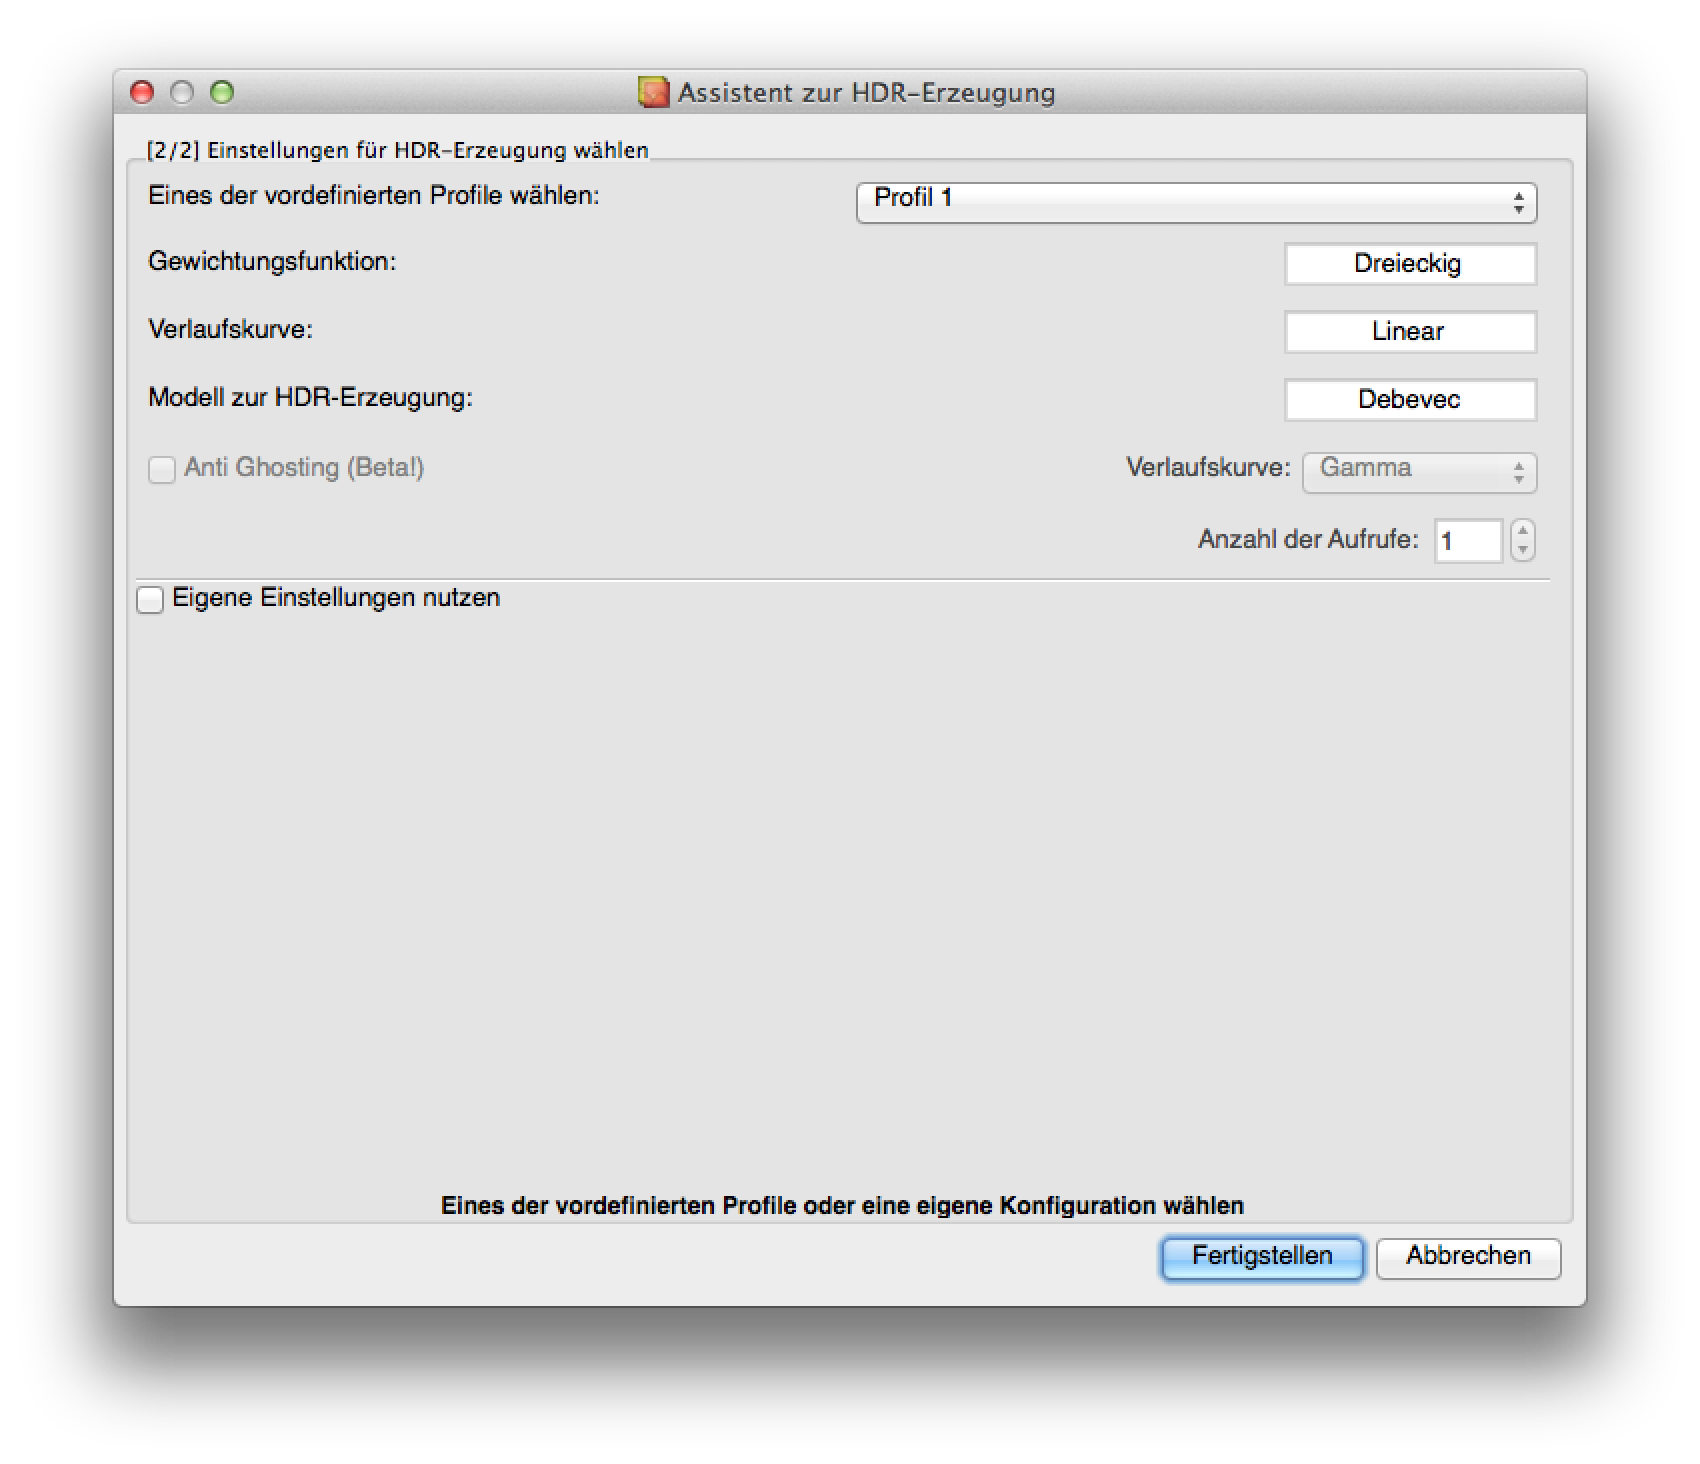
\includegraphics[width=0.8\textwidth]{Luminance}
    \caption{Der Erstell-Assistent von \texttt{Luminance HDR}. Auch hier wird intern der Algorithmus von Debevec und Malik \cite{paper} verwendet.}
    \label{fig:luminance}
  \end{center}
\end{figure}

Darüber hinaus gibt es verschiedene Programme, die speziell auf die Erzeugung von \gls{HDR} Bildern spezialisiert sind (z.B. \texttt{Photomatix}\footnote{\url{http://www.hdrsoft.com/de/}, kostenpflichtig} oder \texttt{Luminance HDR}\footnote{\url{http://qtpfsgui.sourceforge.net}, Freeware}). Der Funktionsumfang dieser Programme ist verhältnismäßig klein, führt jedoch auch Laien schnell zum Ziel, da (wie z.B. bei \texttt{Luminance HDR}, siehe \autoref{fig:luminance}) interaktive Assistenten den Benutzer bei der Erstellung anleiten. 


\begin{figure}
  \begin{center}
    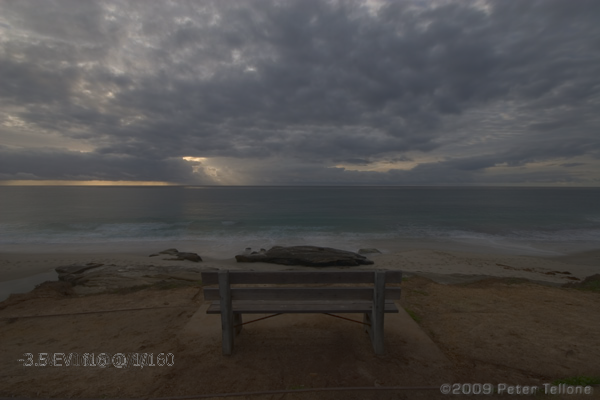
\includegraphics[width=0.8\textwidth]{BenchGeneratedLuminance}
    \caption{Ein mögliches Ergebnis des HDR Bildes. Erstellt mit \texttt{Luminance HDR} und dem \gls{Tone-Mapping} Operator \texttt{Reinhard'05} \cite{Reinhard05}. Bildserie siehe \cite{tellone}.}
    \label{fig:luminance}
  \end{center}
\end{figure}

Als weitere Beispiele für HDR-Software seien hier außerdem \texttt{Dynamic-Photo HDR}\footnote{\url{http://www.mediachance.com/hdri/index.html}, kostenpflichtig} und \texttt{HDR Darkroom}\footnote{\url{http://www.everimaging.com}, kostenpflichtig} genannt. Diese haben sehr viele \gls{Tone-Mapping} Operatoren implementiert und können sowohl realistische als auch sehr verfremdete \gls{HDR} Bilder generieren. 

Ein wirklich einfaches Programm ist \texttt{Picturenaut}\footnote{\url{http://www.hdrlabs.com/picturenaut/}, Freeware}. Die Anzahl und der Funktionsumfang der implementierten \gls{Tone-Mapping} Operatoren ist limitiert, jedoch liefert das Programm recht rasch realitätsgetreue Bilder.


